\documentclass[a4paper, titlepage]{article}

% For equations
\usepackage{amsmath}

% For including figures
\usepackage{graphicx}
\usepackage{float}

% Bibiliography setup
\usepackage[square]{natbib}
\bibliographystyle{agsm}
\usepackage[nottoc]{tocbibind}





% For typesetting matlab
\usepackage{listings}
\usepackage{color} % red, green, blue, yellow, cyan, magenta, black,white
\definecolor{mygreen}{RGB}{28,172,0} % color values Red, Green, Blue
\definecolor{mylilas}{RGB}{170,55,241}

\lstset{language=Matlab,
    basicstyle=\small,
    breaklines=true,
    frame = single,
    morekeywords={matlab2tikz},
    keywordstyle=\color{blue},
    morekeywords=[2]{1}, keywordstyle=[2]{\color{black}},
    identifierstyle=\color{black},
    stringstyle=\color{mylilas},
    commentstyle=\color{mygreen},
    showstringspaces=false,
    numbers=left,
    numberstyle={\tiny \color{black}},% size of the numbers
    numbersep=9pt, % this defines how far the numbers are from the text
    emph=[1]{for,end,break},emphstyle=[1]\color{red}, %some words to emphasise
    %emph=[2]{word1,word2}, emphstyle=[2]{style},    
}


%\title{Assignment 3\\
%System description and analysis\\
%\large EEA004}
%\author{Dan Thilderkvist, Philip Gutierrez}

\begin{document}

%\maketitle

\begin{titlepage}
  \begin{center}
    \vspace*{1cm}
    
\includegraphics[scale=1.0]{../figures/hig_logo_eng.png}\\
    \vspace{1.5cm}
    \large EEA003 - Robotics\\
    \large Assignment 1 Part 1\\
    \vspace{1.5cm}
    Philip Gutierrez\\
    philipgutierrez67@gmail.com\\
    Files: main.m, question1.m\\

    \vspace{1cm}
    Submitted to: Dr. Sajid Rafique and Shaikh Masud Rana\\    
    \vspace{1cm}
    \today
  \end{center}
\end{titlepage}

\tableofcontents
\clearpage



\section{Introduction}


In this assignment we will develop reference frames and rotation matrices for a 2DOF manipulator ahown in figure \ref{fig:axisframes} below.

 
\begin{figure}[h!]
\center
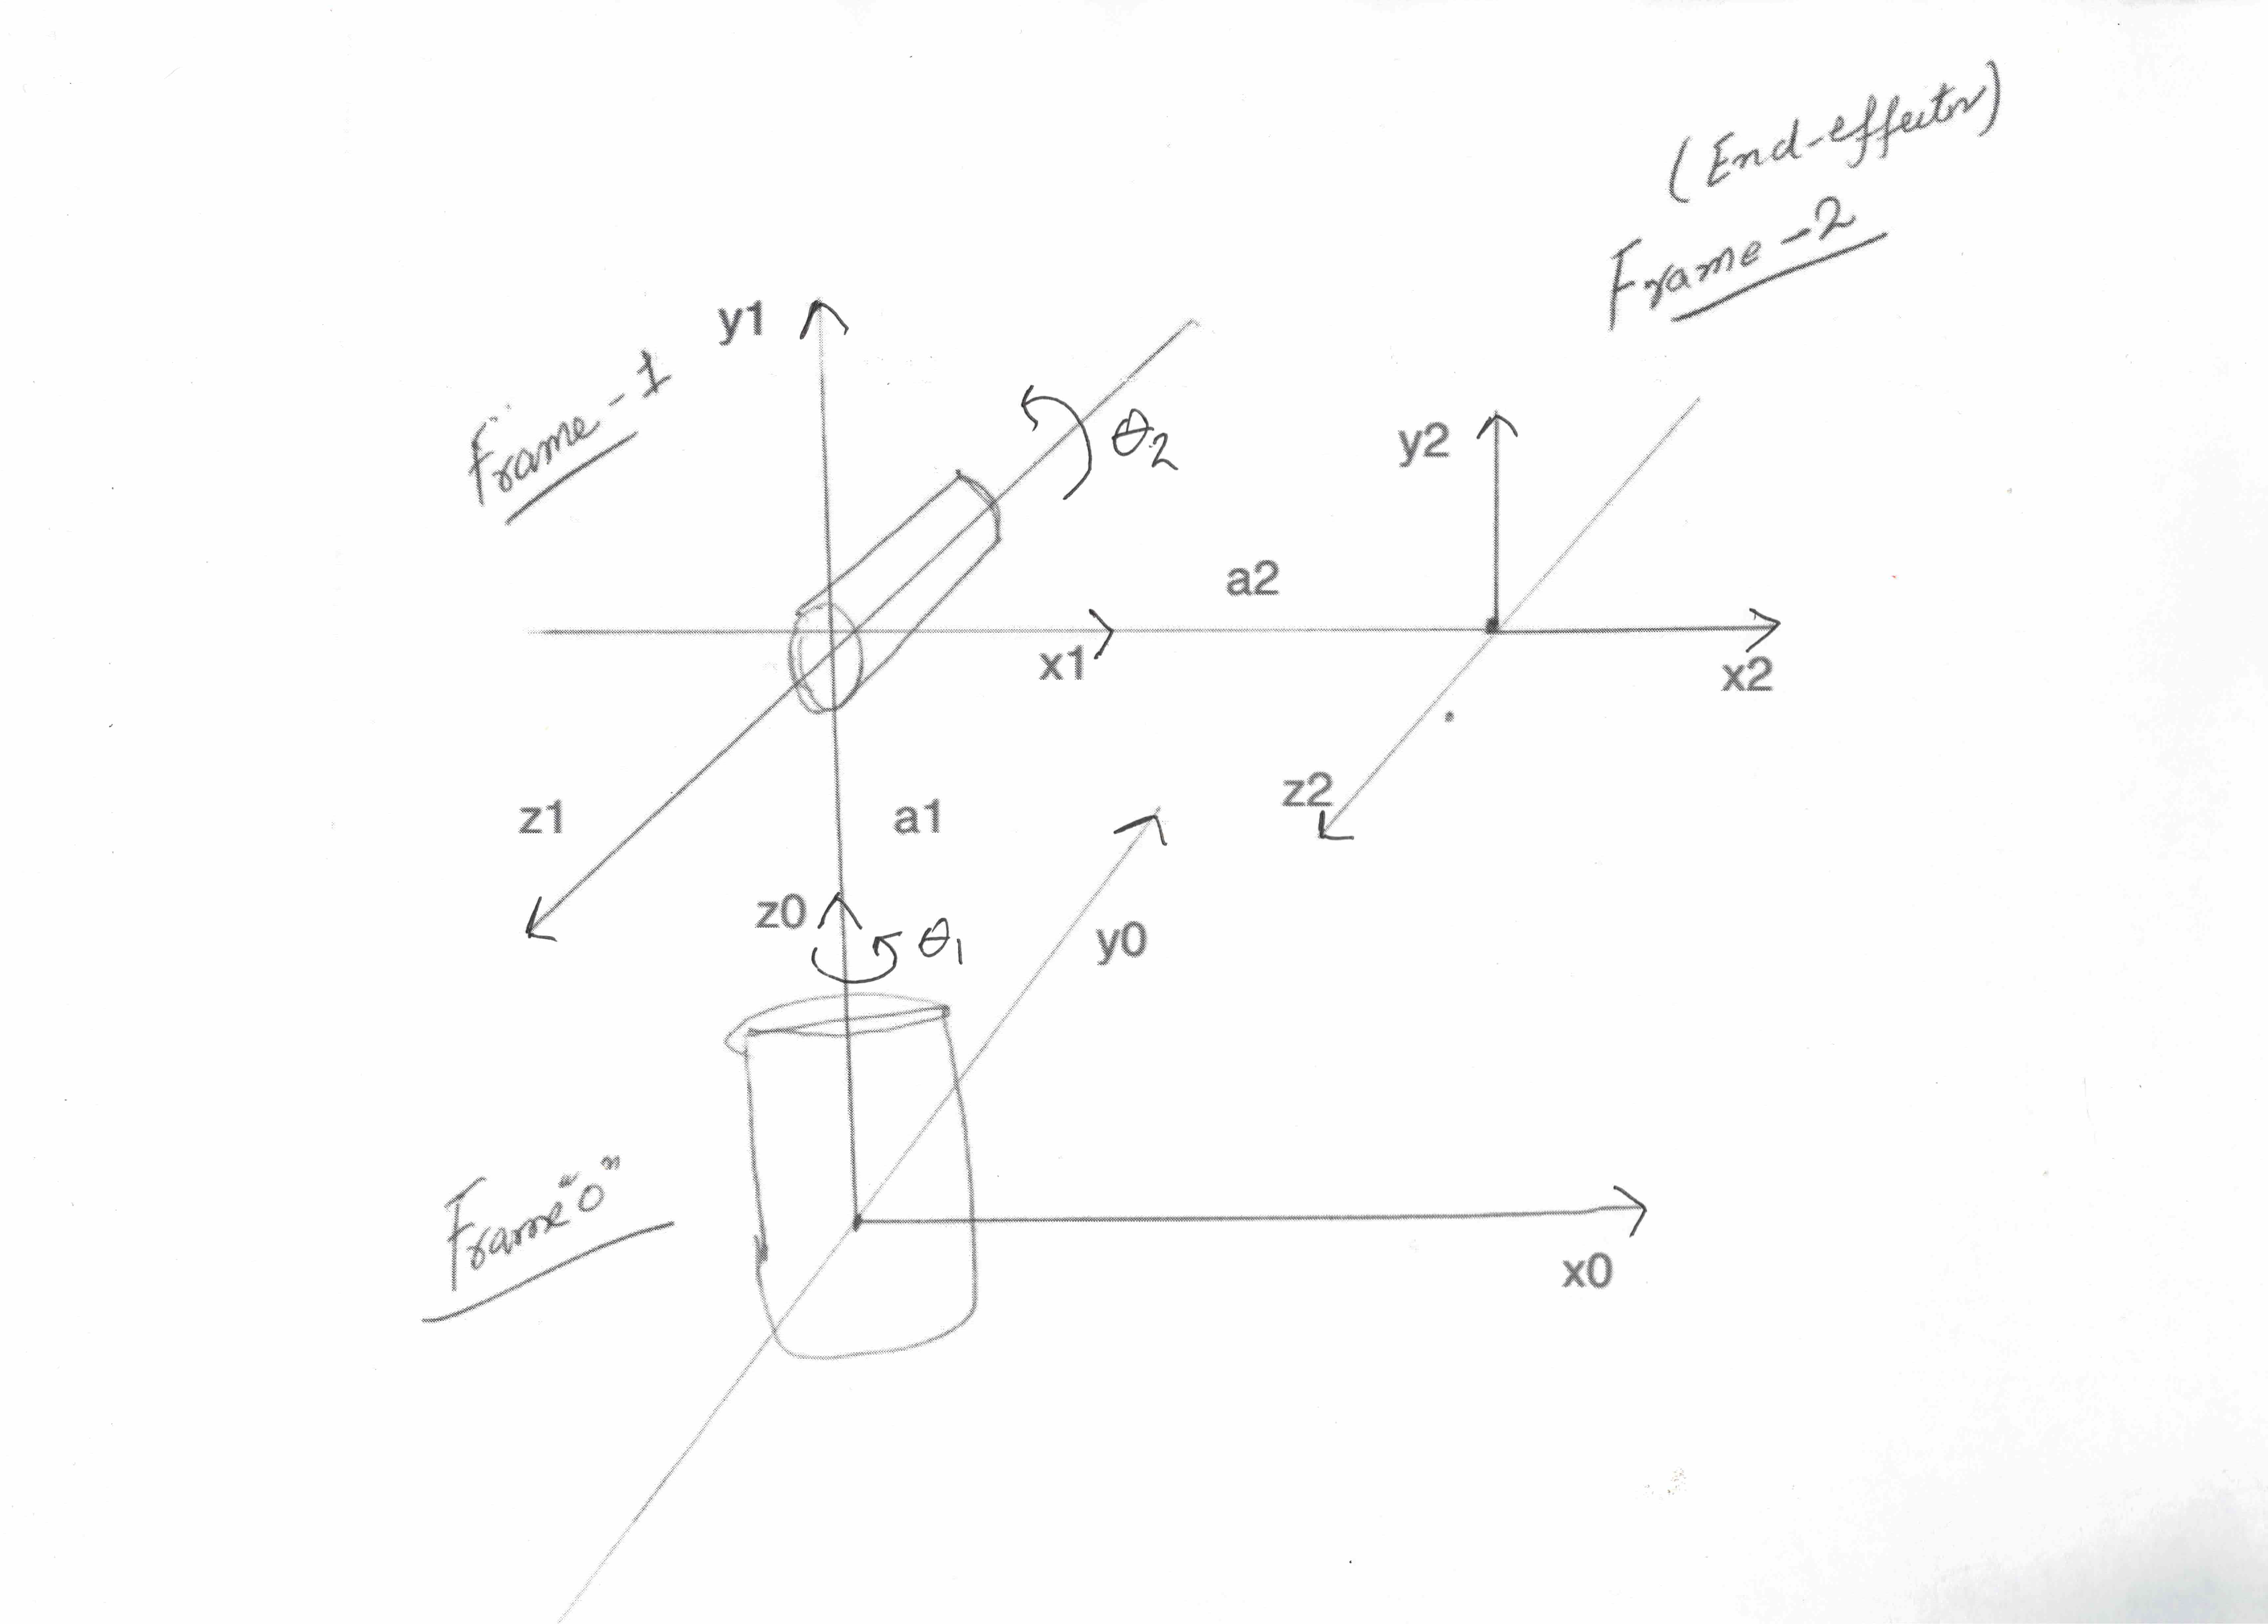
\includegraphics[scale=0.5]{../figures/axisframes.png}
\caption{Axis and Frames.}
\label{fig:axisframes}
\end{figure} 
   

\section{Theory}

The elemental rotation matrices for rotation about the x-, y-, or z-axis are provided as \citep[p.16]{ho90}: 

\begin{equation}
\begin{split}
R_{x}(a)
&=
\begin{bmatrix}
1 & 0 & 0 \\ 0 & cos(a) & -sin(a) \\ 0 & sin(a) & cos(a)
\end{bmatrix}
\end{split}
\end{equation}

\begin{equation}
\begin{split}
R_{y}(b)
&=
\begin{bmatrix}
cos(b) & 0 & sin(b) \\ 0 & 1 & 0 \\ -sin(b) & 0 & cos(b)
\end{bmatrix}
\end{split}
\end{equation}

\begin{equation}
\begin{split}
R_{z}(c)
&=
\begin{bmatrix}
cos(c) & -sin(c) & 0 \\ sin(c) & cos(c) & 0 \\ 0 & 0 & 1
\end{bmatrix}
\end{split}
\end{equation}

A general rotation can be made by multiplying the three elemental matrices (where multiplication is done from right to left)\citep[p.23]{ho90}

\begin{equation}
\begin{split}
R
&= R_{z}(c)R_{y}(b)R_{x}(a)
\end{split}
\end{equation}

\begin{equation}
\begin{split}
R = 
\begin{bmatrix}
cos(c) & -sin(c) & 0 \\ sin(c) & cos(c) & 0 \\ 0 & 0 & 1
\end{bmatrix}
\begin{bmatrix}
cos(b) & 0 & sin(b) \\ 0 & 1 & 0 \\ -sin(b) & 0 & cos(b)
\end{bmatrix}
\begin{bmatrix}
1 & 0 & 0 \\ 0 & cos(a) & -sin(a) \\ 0 & sin(a) & cos(a)
\end{bmatrix}
\end{split}
\end{equation}


A translation vector

\begin{equation}
p = p_{x}\boldsymbol{i} + p_{y}\boldsymbol{j} + p_{z}\boldsymbol{k} 
\end{equation}

can be represented in homogeneous coordinates as\citep[p.12]{ho90}

\begin{equation}
\begin{split}
\boldsymbol{p} = 
\begin{bmatrix}
p_{x} \\ p_{y} \\ p_{z} \\ 1
\end{bmatrix}
\end{split}
\end{equation}

The homogeneous transformation matrix provides a condensed way to represent both the rotation matrix and the translation matrix in a single 4x4 matrix.
The homogeneous transformation matrix is specified as\citep[p.15]{ho90}:

\begin{equation}
\begin{split}
A^1_{2}= 
\begin{bmatrix}
R_{3x3} & p_{3x1} \\  
0_{1x3} &  1_{1x1}
\end{bmatrix}
\end{split}
\end{equation}



\section{Method}

\subsection{Calculating the Rotation Matrix}
To calculate the rotation matrix of the system in figure \ref{fig:axisframes}, we first find the rotation matrix of frame 1 relative frame 0 ($R^0_{1}$), and then the rotation matrix of frame 2 relative frame 1 ($R^1_{2}$).  The resultant rotation matrix is then given by:

\begin{equation}
R^0_{2} = R^0_{1}R^1_{2}
\end{equation}

\subsubsection{Calculating the Rotation Matrix for Frame 1}


Reviewing figure \ref{fig:axisframes} notice that orientation of frame 1 is obtained by rotating 90 degrees around the x-axis, followed by 0 degree rotation about the y-axis and a 0 degree rotation about the z-axis. So, 
\begin{equation}
R^0_{1} = R_{x}(90)R_{y}(0)R_{z}(0)
\end{equation}

\begin{equation}
\begin{split}
R^0_{1} = 
\begin{bmatrix}
1 & 0 & 0 \\ 0 & 0 & -1 \\ 0 & 1 & 0 
\end{bmatrix}
\begin{bmatrix}
1 & 0 & 0 \\ 0 & 1 & 0 \\ 0 & 0 & 1 
\end{bmatrix}
\begin{bmatrix}
1 & 0 & 0 \\ 0 & 1 & 0 \\ 0 & 0 & 1 
\end{bmatrix}
\end{split}
\end{equation}

\begin{equation}
\begin{split}
R^0_{1} = 
\begin{bmatrix}
1 & 0 & 0 \\ 0 & 0 & -1 \\ 0 & 1 & 0 
\end{bmatrix}
\end{split}
\end{equation}

Taking into account the rotation $\theta_{1}$ about the z-axis in figure \ref{fig:axisframes} we get the final rotation matrix for $R^0_{1}(\theta_{1})$ as:

\begin{equation}
R^0_{1}(\theta_{1}) = R_{z}(\theta_{1})R^0_{1}
\end{equation}

\begin{equation}
\begin{split}
R^0_{1}(\theta_{1})
&=
\begin{bmatrix}
cos(\theta_{1}) & -sin(\theta_{1}) & 0 \\ sin(\theta_{1}) & cos(\theta_{1}) & 0 \\ 0 & 0 & 1
\end{bmatrix}
\begin{bmatrix}
1 & 0 & 0 \\ 0 & 0 & -1 \\ 0 & 1 & 0 
\end{bmatrix}
\end{split}
\end{equation}


\begin{equation}
\begin{split}
R^0_{1}(\theta_{1}) = 
\begin{bmatrix}
cos(\theta_{1}) & 0 & sin(\theta_{1})  \\ 
sin(\theta_{1}) & 0 & -cos(\theta_{1})  \\ 
0 & 1 & 0
\end{bmatrix}
\end{split}
\label{equ:r01}
\end{equation}

\subsubsection{Calculating the Rotation Matrix for Frame 2}

Again, reviewing figure \ref{fig:axisframes} notice that orientation of frame 2 is obtained by rotating 0 degrees around the x-axis, followed by 0 degree rotation about the y-axis and a 0 degree rotation about the z-axis. So, 
\begin{equation}
R^1_{2} = R_{x}(0)R_{y}(0)R_{z}(0)
\end{equation}

\begin{equation}
\begin{split}
R^1_{2} = 
\begin{bmatrix}
1 & 0 & 0 \\ 0 & 1 & 0 \\ 0 & 0 & 1 
\end{bmatrix}
\begin{bmatrix}
1 & 0 & 0 \\ 0 & 1 & 0 \\ 0 & 0 & 1 
\end{bmatrix}
\begin{bmatrix}
1 & 0 & 0 \\ 0 & 1 & 0 \\ 0 & 0 & 1 
\end{bmatrix}
\end{split}
\end{equation}

\begin{equation}
\begin{split}
R^1_{2} = 
\begin{bmatrix}
1 & 0 & 0 \\ 0 & 1 & 0 \\ 0 & 0 & 1 
\end{bmatrix}
\end{split}
\end{equation}

Note from figure \ref{fig:axisframes} that reference frame 2 has the same orientation as reference frame 1.  They differ only in a translation, and hence, the results above indicates there is no rotation.

Taking into account the rotation $\theta_{2}$ about the z-axis we get the final rotation matrix for $R^1_{2}(\theta_{2})$ as:

\begin{equation}
R^1_{2}(\theta_{2}) = R_{z}(\theta_{2})R^1_{2}
\end{equation}

\begin{equation}
\begin{split}
R^1_{2}(\theta_{2})
&=
\begin{bmatrix}
cos(\theta_{2}) & -sin(\theta_{2}) & 0 \\ sin(\theta_{2}) & cos(\theta_{2}) & 0 \\ 0 & 0 & 1
\end{bmatrix}
\begin{bmatrix}
1 & 0 & 0 \\ 0 & 1 & 0 \\ 0 & 0 & 1 
\end{bmatrix}
\end{split}
\end{equation}


\begin{equation}
\begin{split}
R^1_{2}(\theta_{2}) = 
\begin{bmatrix}
cos(\theta_{2}) & -sin(\theta_{2}) & 0 \\ 
sin(\theta_{2}) & cos(\theta_{2}) & 0 \\ 
0 & 0 & 1
\end{bmatrix}
\end{split}
\label{equ:r12}
\end{equation}

\subsubsection{Calculating the Complete Rotation Matrix}

The total rotation matrix for the system will depend on $\theta_{1}$ and $\theta_{2}$ and will be:

\begin{equation}
R^0_{2}(\theta_{1},\theta_{2}) = R^0_{1}(\theta_{1})R^1_{2}(\theta_{2})
\label{equ:rotationmatrix}
\end{equation}


\subsection{Calculating the Translation Matrix}

From figure \ref{fig:axisframes} note that the position of Frame 1 is simply translated along the $z_{0}$ axis of Frame 0.  There is no translation along the $x_{0}$ or $y_{0}$ axis, so the translation matrix becomes:

\begin{equation}
\begin{split}
p^0_{1} = 
\begin{bmatrix}
0 \\ 
0 \\ 
a_{1}
\end{bmatrix}
\end{split}
\label{equ:p01}
\end{equation}

Note also from figure \ref{fig:axisframes} that the position of Frame 2 is  translated along the $x_{1}$ axis of Frame 1, and that it's position will depend on $\theta_{2}$.  The translation matrix becomes:

\begin{equation}
\begin{split}
p^1_{2} = 
\begin{bmatrix}
a_{2}cos(\theta_{2}) \\ 
a_{2}sin(\theta_{2}) \\ 
0
\end{bmatrix}
\end{split}
\label{equ:p12}
\end{equation}

The resulting translation matrix for the system becomes:

\begin{equation}
\begin{split}
p^0_{2} = p^0_{1} + p^1_{2} \\ 
p^0_{2} = 
\begin{bmatrix}
a_{2}cos(\theta_{2}) \\ 
a_{2}sin(\theta_{2}) \\ 
a_{1}
\end{bmatrix}
\end{split}
\label{equ:translationmatrix}
\end{equation}

 

\subsection{Calculating the Transformation Matrix}

The transformation matrix is defined as \citep[p.15]{ho90}:

\begin{equation}
\begin{split}
A^0_{1}= 
\begin{bmatrix}
R^0_{1} & p^0_{1} \\  
0_{1x3} &  1_{1x1}
\end{bmatrix}
\end{split}
\label{equ:transmatrix}
\end{equation}

Using \ref{equ:r01} and \ref{equ:p01} from above and inserting into \ref{equ:transmatrix} we get:

\begin{equation}
\begin{split}
A^0_{1}(\theta_{1}) = 
\begin{bmatrix}
cos(\theta_{1}) & 0 & sin(\theta_{1}) & 0 \\ 
sin(\theta_{1}) & 0 & -cos(\theta_{1}) & 0  \\ 
0 & 1 & 0 & a_{1} \\
0 & 0 & 0 & 1
\end{bmatrix}
\end{split}
\label{equ:a01}
\end{equation}

Using \ref{equ:r12} and \ref{equ:p12} from above and inserting into \ref{equ:transmatrix} we get:


\begin{equation}
\begin{split}
A^1_{2}= 
\begin{bmatrix}
R^1_{2} & p^1_{2} \\  
0_{1x3} &  1_{1x1}
\end{bmatrix}
\end{split}
\end{equation}

\begin{equation}
\begin{split}
A^1_{2}(\theta_{2}) = 
\begin{bmatrix}
cos(\theta_{2})  & -sin(\theta_{2}) & 0 & a_{2}cos(\theta_{2})\\ 
sin(\theta_{2})  & cos(\theta_{2}) & 0  & a_{2}sin(\theta_{2})\\ 
0 & 0 & 1 & 0 \\
0 & 0 & 0 & 1
\end{bmatrix}
\end{split}
\label{equ:a12}
\end{equation}

The complete transformation matrix is provided \citep[p.23]{ho90} as:

\begin{equation}
\begin{split}
A^0_{2}(\theta_{1},\theta_{2}) = A^0_{1}(\theta_{1})A^1_{2}(\theta_{2}) 
\end{split}
\label{equ:a02}
\end{equation}



\subsection{Identifying the Denavit-Hartenberg Parameters}

The Denavit-Hartenberg parameters may be identified by following the following guidelines \citep[p.21]{ho90}

$\theta_{i}$ : the angle between the $x_{i-1}$ and the $x_{i}$ axis as measured along the $z_{i-1}$ axis.

$d_{1}$ : the distance between the origin of the $(i-1)^th$ coordinate system and the intersection point of the $z_{i-1}$ axis with the $x_{i}$ axis.

$a_{i}$ : the common normal distance between the $(i-1)^th$ and the $i^th$ joints.

$\alpha_{i}$ : the angle between the $z_{i-1}$ and the $z_{i}$ axis as measured along the $x_{i}$ axis.

Based on figure \ref{fig:axisframes} we can identify the following parameters:

\begin{center}
\begin{tabular}{||c c c c c||} 
 \hline
 Frame & $\theta$ & $\alpha$ & r & d \\ [0.5ex] 
 \hline\hline
 1 & $\theta_{1}$ & 90 & 0 & $a_{1}$ \\
 \hline
2 & $\theta_{2}$ & 0 & $a_{2}$ & 0 \\
 \hline
 \hline
\end{tabular}
\end{center}

\section{Results}
\subsubsection{Calculate the Rotation Matrix}

From \ref{equ:r01} we have:

\begin{equation}
\begin{split}
R^0_{1}(\theta_{1}) = 
\begin{bmatrix}
cos(\theta_{1}) & 0 & sin(\theta_{1})  \\ 
sin(\theta_{1}) & 0 & -cos(\theta_{1})  \\ 
0 & 1 & 0
\end{bmatrix}
\end{split}
\end{equation}

From \ref{equ:r12} we have:


\begin{equation}
\begin{split}
R^1_{2}(\theta_{2}) = 
\begin{bmatrix}
cos(\theta_{2}) & -sin(\theta_{2}) & 0 \\ 
sin(\theta_{2}) & cos(\theta_{2}) & 0 \\ 
0 & 0 & 1
\end{bmatrix}
\end{split}
\end{equation}

From \ref{equ:rotationmatrix} we have:

\begin{equation}
R^0_{2}(\theta_{1},\theta_{2}) = R^0_{1}(\theta_{1})R^1_{2}(\theta_{2})
\end{equation}


\subsubsection{Calculate the Translation Matrix}

From \ref{equ:p01}, \ref{equ:p12}, and \ref{equ:translationmatrix} we have:

\begin{equation}
\begin{split}
p^0_{1} = 
\begin{bmatrix}
0 \\ 
0 \\ 
a_{1}
\end{bmatrix}
\end{split}
\end{equation}

\begin{equation}
\begin{split}
p^1_{2} = 
\begin{bmatrix}
a_{2}cos(\theta_{2}) \\ 
a_{2}sin(\theta_{2}) \\ 
0
\end{bmatrix}
\end{split}
\end{equation}


\begin{equation}
\begin{split}
p^0_{2} = 
\begin{bmatrix}
a_{2}cos(\theta_{2}) \\ 
a_{2}sin(\theta_{2}) \\ 
a_{1}
\end{bmatrix}
\end{split}
\end{equation}


\subsubsection{Calculate the Transformation Matrix}

From \ref{equ:a01}, \ref{equ:a12}, and \ref{equ:a02} we have:

\begin{equation}
\begin{split}
A^0_{1}(\theta_{1}) = 
\begin{bmatrix}
cos(\theta_{1}) & 0 & sin(\theta_{1}) & 0 \\ 
sin(\theta_{1}) & 0 & -cos(\theta_{1}) & 0  \\ 
0 & 1 & 0 & a_{1} \\
0 & 0 & 0 & 1
\end{bmatrix}
\end{split}
\end{equation}


\begin{equation}
\begin{split}
A^1_{2}(\theta_{2}) = 
\begin{bmatrix}
cos(\theta_{2})  & -sin(\theta_{2}) & 0 & a_{2}cos(\theta_{2})\\ 
sin(\theta_{2})  & cos(\theta_{2}) & 0  & a_{2}sin(\theta_{2})\\ 
0 & 0 & 1 & 0 \\
0 & 0 & 0 & 1
\end{bmatrix}
\end{split}
\end{equation}


\begin{equation}
\begin{split}
A^0_{2}(\theta_{1},\theta_{2}) = A^0_{1}(\theta_{1})A^1_{2}(\theta_{2}) 
\end{split}
\end{equation}



\subsubsection{Calculate the DH-parameters}

From section 3.4 we have:

\begin{center}
\begin{tabular}{||c c c c c||} 
 \hline
 Frame & $\theta$ & $\alpha$ & r & d \\ [0.5ex] 
 \hline\hline
 1 & $\theta_{1}$ & 90 & 0 & $a_{1}$ \\
 \hline
2 & $\theta_{2}$ & 0 & $a_{2}$ & 0 \\
 \hline
 \hline
\end{tabular}
\end{center}


\clearpage
\bibliography{reference}

\clearpage
\appendix

\section{Appendix}
Here is the Matlab code used to generate the results in the report and the figures.

\lstinputlisting{../code/main.m}
\lstinputlisting{../code/question1.m}
\lstinputlisting{../code/question2.m}

\end{document}